\documentclass{exam}
\usepackage[utf8]{inputenc}

\usepackage[frenchb]{babel}
\usepackage[T1]{fontenc}

\usepackage{graphicx}
\usepackage{amssymb}
\usepackage{amsmath}
\usepackage{wasysym} %smiley
\usepackage{hyperref}% hyperliens
\usepackage{tikz}
\usetikzlibrary{babel,positioning,calc}
\usepackage[]{circuitikz}
\usepackage{textcomp}
\usepackage[long]{datetime}
\usepackage{minted}
\usepackage{gensymb} % \ohm, celsius
\usepackage{framed}
\usepackage{pdfpages}
\usepackage{todonotes}
\usepackage{multirow}
\usepackage{wrapfig}
\usepackage{pgfplots}
\usepackage{subcaption} % subfigure
\usepackage{siunitx} 
\usepackage{circuitikz}


\langexam{frenchb}

\newboolean{koriG}
\ifx\koriG\undefined
\correction{false}
\else
\correction{true}
\fi

\author{DLH}

\toptitle{[3bepe3U] Mesures}{1re Session 2022-2023}

\changedate{18}{01}{2023}

% \correction{false}
% \correction{true}

\begin{document}

\examtitle{Examen de Mesures}{~}
\frontpage{Consignes.tex}
\vfill
\namebox{id}
\newpage






%%%%%%%%%%%%%%%%%%%%%%%%%%%%%%%%%
% ADC
%%%%%%%%%%%%%%%%%%%%%%%%%%%%%%%%%
\section{ADC}


\Question{3}{1}
{
	À l'issue d'une conversion d'une tension analogique en un \textit{bitstream} dans un ADC Delta-Sigma, vous obtenez le train suivant~: \texttt{101011001110}. Sachant que votre circuit est alimenté en $\pm 3 V$, quelle est la tension d'entrée ainsi convertie ?
}
{
	$\frac{7}{12} \cdot 6 - 3 = 0.5 V$.
}

Vous utilisez ensuite l'ADC dont la figure suivante se trouve dans une vieille datasheet~:
\begin{center}
	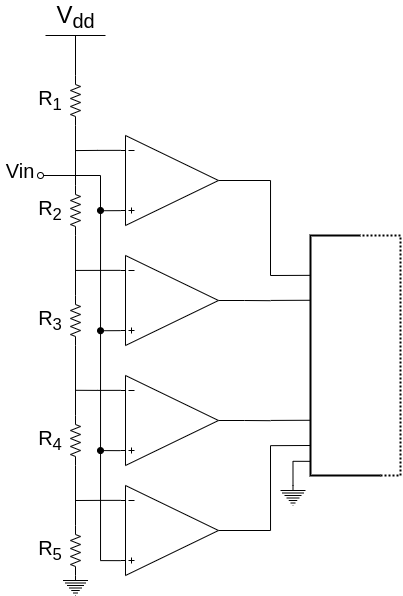
\includegraphics[width=.3\paperwidth]{flash.png}
\end{center}
Malheureusement, il vous manque la partie droite du schéma.

\clearpage
\Question{2}{1}
{
	De quel type de convertisseur s'agit-il ?
	À quoi le reconnaissez-vous ?
}
{
	ADC Flash. On le reconnait à la cascade de comparateurs et les diviseurs de tension permettant de régler les tensions de seuil.
}

\Question{3}{1}
{
	Combien de bits sont nécessaires pour représenter les valeurs analogiques converties ?
}
{
	Étant donné qu'on a 5 entrées possibles, il faut 3 bits pour les représenter. Certains codes ne seront simplement pas utilisés.
}

\Question{2}{1}
{
	Quelle est la résolution de ce convertisseur ?
}
{
	En théorie, la résolution d'un convertisseur sur 3 bits serait de $V_{dd}/2^3$, soit $V_{dd}/8$.
	Cependant, cette architecture ne divise la tension d'entrée qu'en 5 valeurs différentes étant donné qu'il n'y a que 4 comparateurs. La résolution est donc de $V_{dd}/5$.
}

\Question{2}{1}
{
	Quelle est la valeur des différentes résistances ?
}
{
	Elles ont toutes la même valeur et cette valeur n'a pas d'importance.
}

\clearpage




%%%%%%%%%%%%%%%%%%%%%%%%%%%%%%%%%
% DAC
%%%%%%%%%%%%%%%%%%%%%%%%%%%%%%%%%
\section{Erreur de conversion}
Vous souhaitez utiliser un DAC sur 3 bits dont la résolution est de 0.5 V et décidez d'abord de le caractériser afin de vérifier son bon fonctionnement.

\Question{1}{1}
{
Tracez ci-dessous la fonction de transfert \textbf{idéale} d'un DAC.
\begin{center}
	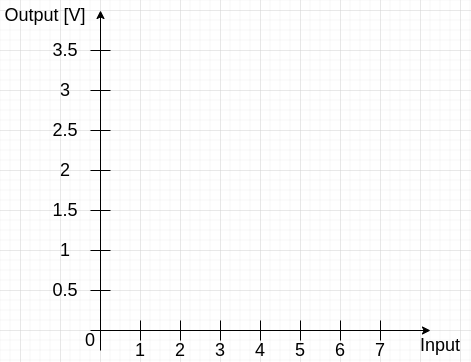
\includegraphics[width=.3\paperwidth]{erreur-conversion_axes.png}
\end{center}
\vspace*{-2cm}
}
{
	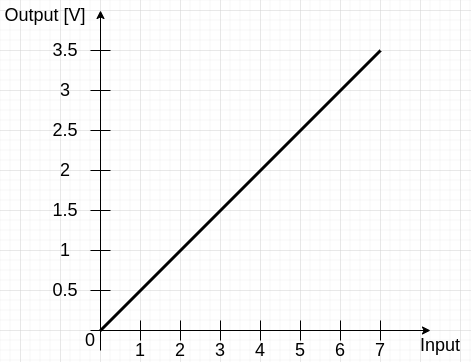
\includegraphics[width=.4\paperwidth]{erreur-conversion_axes_ideal.png}
}

\Question{4}{3}
{
Vous obtenez finalement le relevé suivant. 
Mettez en évidence les erreurs de conversion et décrivez-les.
\begin{flushleft}
	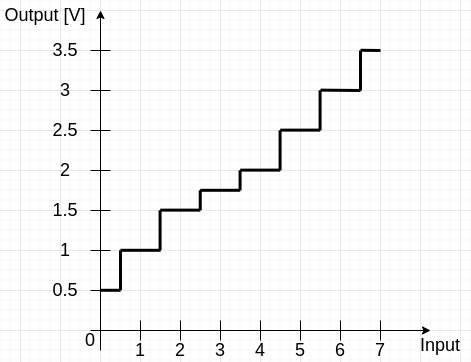
\includegraphics[width=.35\paperwidth]{erreur-conversion.png}
\end{flushleft}
}
{
	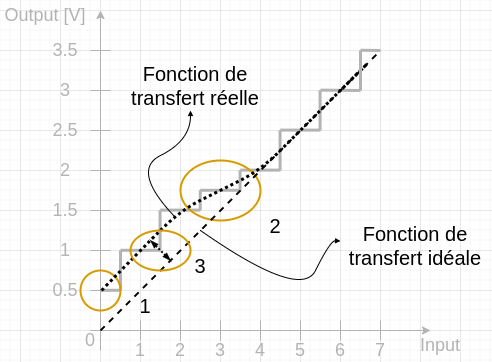
\includegraphics[width=.4\paperwidth]{erreur-conversion_correction.png}
	On peut observer \textbf{trois} erreurs différentes.
	\begin{enumerate}
		\item Offset, la fonction de transfert ne commence pas à 0.
		\item Non-linéarité différentielle (DNL), un code binaire ne représente pas la même variation de tension. Dans les deux cas, le DNL est de -0.5LSB.
		\item Non-linéarité intégrale (INL), on peut mettre en évidence un écart entre la fonction de transfert idéale et la fonction de transfert réelle passant au centre de chaque pas de conversion.
	\end{enumerate}
}

\clearpage




%%%%%%%%%%%%%%%%%%
% Oscilloscope
%%%%%%%%%%%%%%%%%%
\section{Configuration de l'oscilloscope}
Vous souhaitez observer la tension $V_{\mbox{charge}}$ en sortie d'un montage redresseur double alternance avec capacité de filtrage.
\begin{center}
\begin{circuitikz}\draw
	(-2,1) to [sV, l_=$V_{ac}$] (-2,3)
	(-2,1) to (-1,1) to (-1,1.75) to [short,-*](2,1.75)
	(-2,3) to (-1,3) to (-1,2.25) to [short,-*](0,2.25)
	(0,0) to [Do] (0,2) to [Do](0,4)
	(2,0) to [Do,*-] (2,2) to [Do, -*](2,4)
	(0,4) to [short](5,4)
	(0,0) to [short](2,0)
	(5,4) to [european resistor,l=$Z_{Ch}$] (5,0) to (2,0)
	(4,4) to [eC,l_=$C$, *-*] (4,0)
	(6,4) to [open, v^<=$V_{\mbox{charge}}$] (6,0)
;\end{circuitikz}
\end{center}

Vous obtenez le relevé suivant à l'aide de l'oscilloscope du laboratoire~:
\begin{center}
	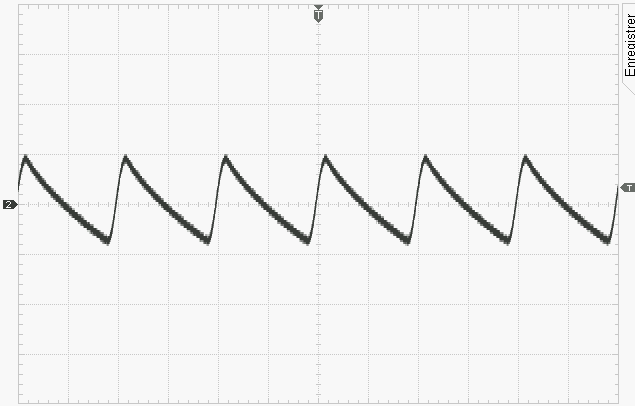
\includegraphics[width=.4\paperwidth]{rectified.png}
\end{center}

\Question{4}{3}
{
	Sachant que $V_{ac}$ a une fréquence de 100~Hz et que $V_{\mbox{charge}}$ a une amplitude de 200~mV crête-à-crête, comment l'oscilloscope a-t-il été configuré ?
}
{
	100mV/div, 5ms/div (il s'agit d'un redresseur \textit{double} alternance) et couplage AC pour centrer la partie alternative de la trace.
}

\Question{6}{2}
{
	Comment pourriez-vous configurer l'oscilloscope pour capturer un événement \textbf{sporadique} {\footnotesize (irrégulier, non-périodique)} durant quelques nanosecondes ?
}
{
	L'élément essentiel est le \textbf{trigger} à configurer correctement. Étant donné qu'il ne s'agit pas d'un événement périodique, on va le configurer en mode \textbf{single}. Le type de déclenchement peut par exemple être une pente montante classique, avec un seuil de déclenchement correspondant à la moitié de la pente montante qu'on souhaite afficher.

	Il s'agit ensuite de configurer correctement \textbf{les échelles de temps et de tension} afin d'afficher l'entièreté du signal lors de sa capture.
}

\clearpage






\section{Fabrication de PCB}
Vous travaillez pour une entreprise fabriquant des PCB.
Un de vos client vous envoie un design ainsi qu'une série de tests à effectuer afin de vérifier la fabrication et l'assemblage de la carte électronique.
Votre client a sélectionné les tests suivants~:
\begin{itemize}
	\item Functional Circuit Testing
	\item Automated X-ray Inspection
	\item Visual Inspection
	\item Flying Probe Testing
\end{itemize}
~\newline{}


\Question{5}{2}
{
	Dans quel ordre allez-vous effectuer ces quatre tests ? Le but est de détecter des erreurs de fabrication le plus rapidement possible et de façon la plus économique.
}
{
	Voici l'ordre des tâches à effectuer :
	\begin{enumerate}
		\item Visual Inspection, cette inspection ne demande pas de configuration particulière et peut être effectuée très tôt dans le processus de fabrication. Il s'agit de la vérification de base.
		\item Automated X-ray Inspection, bien que cette vérification demande du matériel spécialisé, on peut supposer que votre entreprise possède déjà l'appareil puisqu'elle propose ses services. Sa configuration peut néanmoins demander davantage de manipulation qu'une simple inspection visuelle.
		\item Flying Probe Testing, nécessite une configuration unique à la carte testée. De plus elle est relativement lente, occupant la machine pendant un temps précieux.
		\item Functional Circuit Testing, nécessite non seulement un configuration unique à la carte, mais aussi un circuit complètement assemblé. Elle ne peut être effectuée qu'en fin de chaîne et prend plus de temps que les autres vérifications.
	\end{enumerate}


}


\Question{4}{2}
{
	En quoi consiste le \textit{Flying Probe Testing} ?
}
{
	Une série de sondes mobiles se déplacent automatiquement pour mesurer différentes grandeurs au sein du circuit (généralement des tensions).
	Le test a beau être automatisé, il reste trop lent pour tester une production de masse et n'est pas capable de détecter certains défauts.
	Il reste moins cher que d'autres alternatives, comme le ICT et n'est pas limité à une prise de mesure uniquement aux points de test.
}


\Question{6}{2}
{
	Le client vous demande finalement d'effectuer un \textit{Burn-in Testing} en plus des autres tests. Cette requête modifie-t-elle votre procédure ? Quels sont les risques qui y sont associés ?
}
{
	Le burn-in testing sera effectué \textbf{en dernier lieu}, une fois qu'on s'est assuré de son bon fonctionnement.
	Il faut néanmoins que le client soit conscient que ce test peut \textbf{réduire la durée de vie} du produit et induit un \textbf{surcoût} certain à sa commande.
}
\clearpage


\section{Multimètre}
Vous trouverez ci-après un extrait de la datasheet du multimètre \texttt{IDM72}.


\Question{2}{1}
{
Quelle est la plus petite valeur de résistance pouvant être affichée ?
}
{
	Plus petit calibre : $600\Omega$. Affichage « 6000 count », donc la valeur la plus faible pouvant être affichée est $0.1\Omega$.
}

\Question{3}{2}
{
Vous mesurez une résistance dont la valeur affichée par le multimètre est de 100 $\Omega$.
Quelle est l'incertitude sur cette mesure ?
}
{
	Le calibre utilisé est de $600\Omega$, donc la précision est de $\pm(0.7\%+2\mbox{dgt})$, soit $100\Omega \pm (0.7\Omega + 0.2 \Omega)$, 2 digits correspondant à $0.2 \Omega$.
	L'incertitude est donc de $0.9\Omega$.
}

\Question{5}{2}
{
	Vous mesurez une tension continue de 100 mV aux bornes d'une résistance de $1 M\Omega$.
	Quelle est la tension réelle aux bornes de la résistance ?
}
{
	Sans autre information sur la topologie du circuit, on peut supposer que \textbf{la résistance d'entrée du multimètre n'a pas d'influence}. Le mesure étant prise en parallèle de la résistance, une mesure de 100 mV correspond à la même tension aux bornes cette dernière.
	On peut néanmoins prendre en compte l'incertitude de mesure du voltmètre de tension continue : $\pm(0.9\%+5\mbox{dgt})$. Pour mesurer 100 mV, l'appareil sera réglé sur le calibre « 600 mV », donc 1 digit correspond à 0.1 mV.
	On obtient ainsi une incertitude de $\pm(0.9 mV + 0.5 mV)$, soit \textbf{$\pm 1.4 mV$}.
}

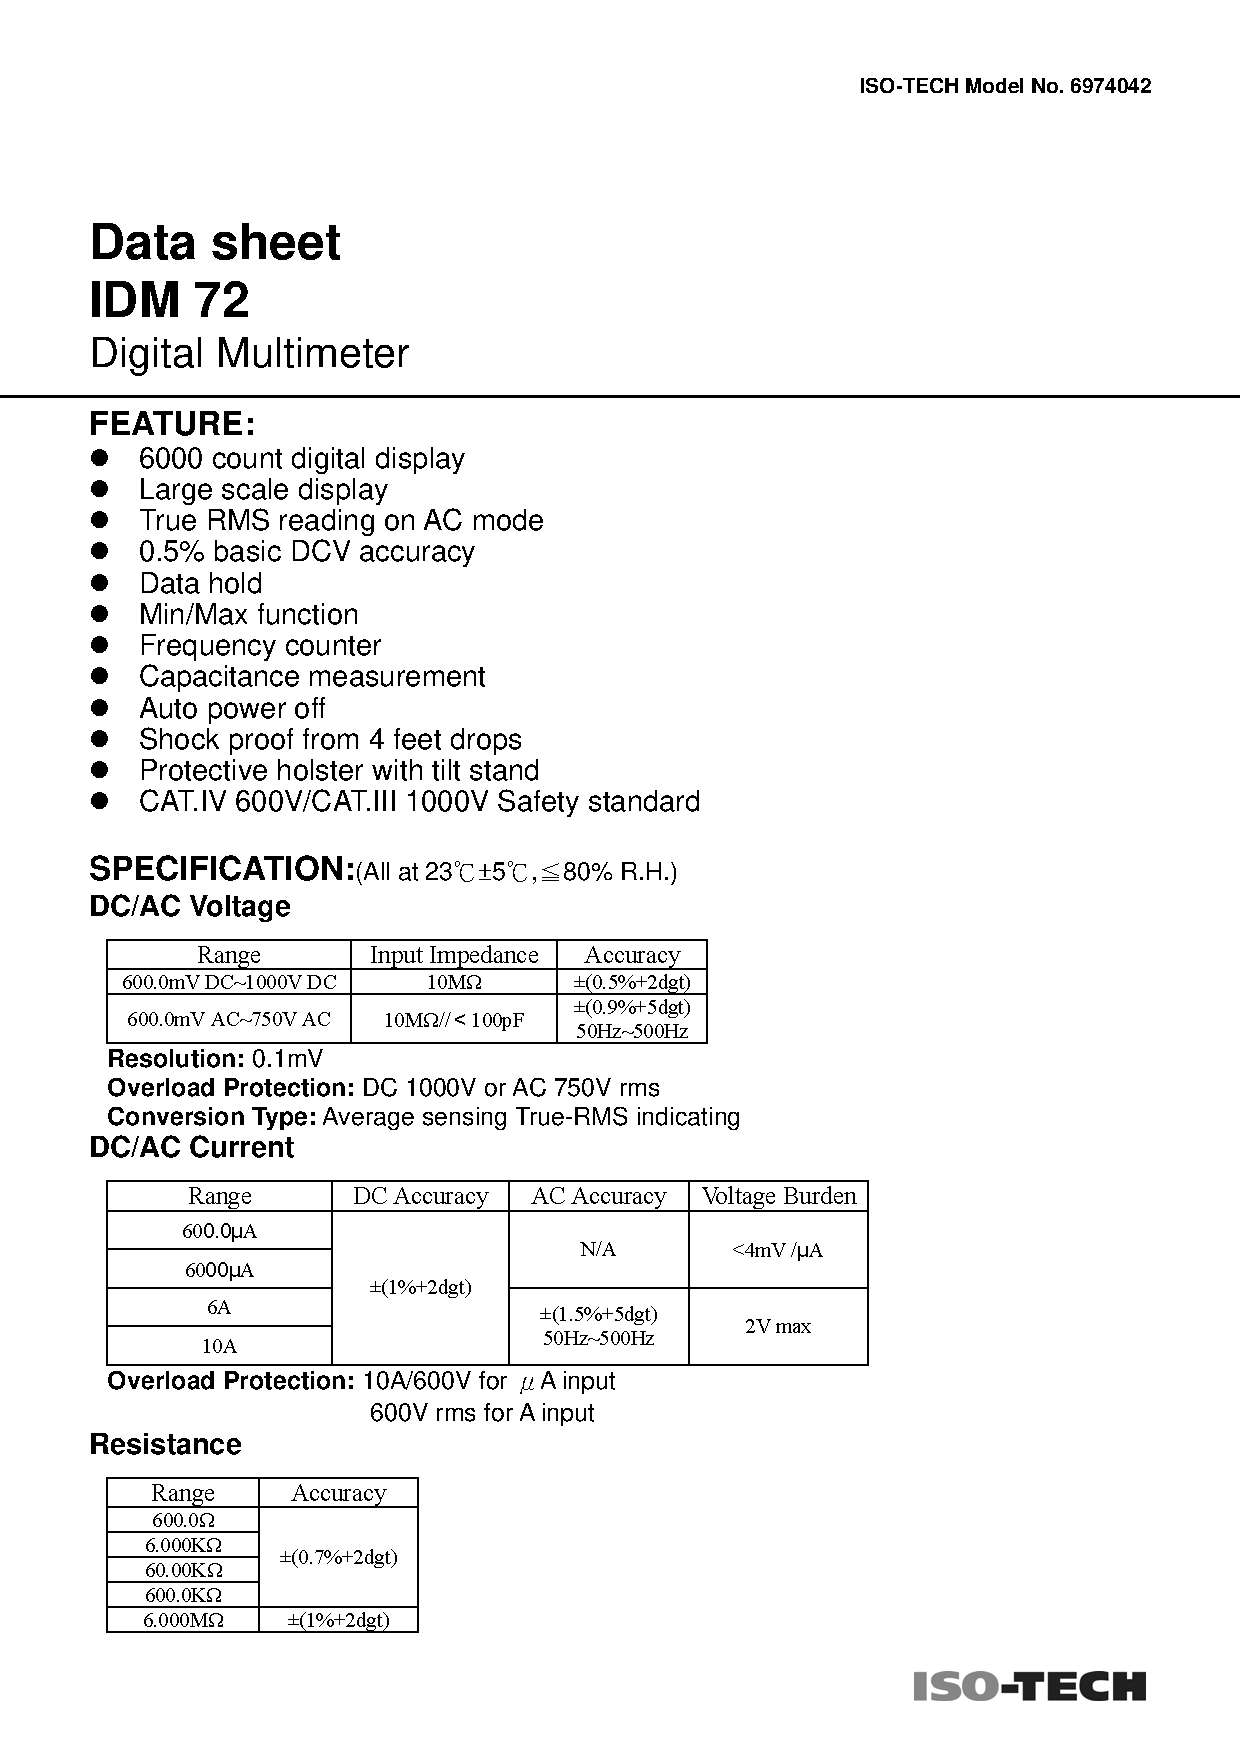
\includepdf[pages={1}]{IDM72.pdf}\label{pdf:idm72}
\clearpage

\adddraft{1}{grid}
%\adddraft{1}{}

\end{document}
